\documentclass[11pt, twoside]{article}
\usepackage[francais]{babel}
\usepackage[T1]{fontenc}
\usepackage[latin1]{inputenc}
\usepackage[left=5mm, right=5mm, top=3mm, bottom=3mm]{geometry}
\usepackage{float}
\usepackage{graphicx}
\usepackage{array}
\usepackage{multirow}
\usepackage{amsmath,amssymb,mathrsfs}
\usepackage{soul}
\usepackage{textcomp}
\usepackage{eurosym}
 \usepackage{variations}
\usepackage{tabvar}


\pagestyle{empty}

\begin{document}

\begin{center}
\Large{\textbf{Devoir maison 3}}
\end{center}

\enskip




\begin{center}
\fbox{
\begin{minipage}{19cm}
\textit{Devoir � rendre sur feuille grand format pour le
\textbf{jeudi 9 janvier 2013}. Pensez � bien r�diger  toutes vos
r�ponses.}
\end{minipage}
}
\end{center}

\enskip

\ul{Exercice 1}: (\textit{4 points})



\begin{tabular}{cc}
\begin{minipage}{12cm}
En utilisant les informations de la figure ci-contre, calculer les longueurs BE
et CA.


L'unit� est le centim�tre, la figure n'est pas � l'�chelle.
\end{minipage}

&
\begin{minipage}{6cm}
\begin{center}
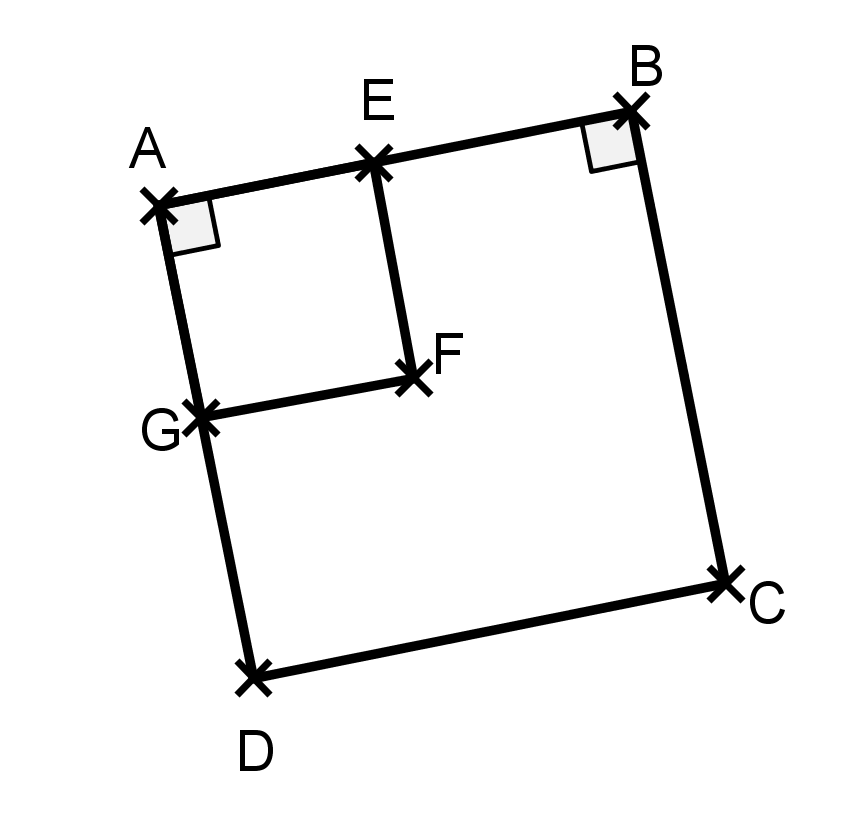
\includegraphics[width=4cm]{images/ex1.png}
\end{center}
\end{minipage} 
\end{tabular}

\bigskip

\ul{Exercice 2}: (\textit{6 points})



\begin{tabular}{cc}
\begin{minipage}{15cm}
OAB est un triangle rectangle en A. D appartient � la droite (OB) et C
appartient � la droite (OA). On donne en millim�tres: OC=28; OD=35; CD=21;
OA=42.
\end{minipage}

&
\begin{minipage}{4cm}
\begin{center}
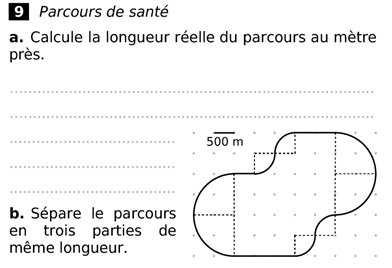
\includegraphics[width=4cm]{images/ex2.jpg}
\end{center}
\end{minipage} 
\end{tabular}


\begin{enumerate}
  \item Montrer que le triangle ODC est rectangle en C.
  \item Que peut-on dire des droites (DC) et (AB)? Justifier votre r�ponse.
  \item Calculer les longueurs OB et AB.
\end{enumerate}

\bigskip

\ul{Exercice 3}: (\textit{6,5 points})

\begin{tabular}{cc}
\begin{minipage}{15cm}
La figure ci-contre n'est pas en vraie grandeur. Le quadrilat�re BREV est un
rectangle avec BR=13 cm et BV=7,2 cm. Le point T est sur le segment [VE] tel
que VT=9,6 cm. N est le point d'intersection des droites (BT) et (RE).
\end{minipage}

&
\begin{minipage}{4cm}
\begin{center}
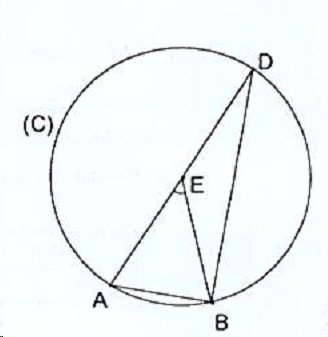
\includegraphics[width=35mm]{images/ex3.jpg}
\end{center}
\end{minipage} 
\end{tabular}


\begin{enumerate}
  \item Montrer que TE=3,4 cm.
  \item Calculer la longueur BT.
  \item Calculer la longueur EN.
  \item Calculer la longueur TN.
\end{enumerate}


\bigskip

\ul{Exercice 4}: (\textit{6 points}) \qquad D�velopper puis r�duire les
expressions suivantes:

\begin{tabular}{ll}
\quad & \quad \\
\qquad \qquad $A=(9a-3)(8-7a)-(3a-5)$  \qquad \qquad & \qquad \qquad
$B=2+3u(-7+4u^2)+(-8u^3+4)$ \\

\quad &\quad \\
\qquad \qquad $C=5y(10-4y)+(-6+8y)(y-7)$  \qquad \qquad & \qquad \qquad 
$D=7-(2t+3)(-4t-5)$

\end{tabular}

\bigskip

\ul{Exercice 5}: (\textit{4 points}) \qquad Factoriser au maximum les
expressions suivantes:

\enskip

$E=20y^2-4y$ \qquad \quad $F=18-72w$ \qquad \quad $G=-3d^3+21d^2$ \qquad \quad 
$H=(9z+3)(3z-1)-2(9z+3)$

\bigskip

\ul{Exercice 6}: (\textit{3,5 points}) \qquad Voici un programme de calcul:

\begin{center}
\fbox{
\begin{minipage}{12cm}
\begin{enumerate}
  \item [$\bullet$] Choisir un nombre n.
  \item [$\bullet$] Lui ajouter 7.
  \item [$\bullet$] Multiplier le r�sultat par 3.
  \item [$\bullet$] Soustraire le triple du nombre choisi au r�sultat.
\end{enumerate}
\end{minipage}}

\end{center}

\begin{enumerate}
  \item Effectuer ce programme pour n=8.
  \item Effectuer ce programme pour deux autres valeurs de n (de votre choix)
  et �crire vos calculs.
  \item Quelle conjecture peut-on faire? (C'est-�-dire que remarquez-vous?)
  D�montrer votre conjecture.
\end{enumerate}
\end{document}
